% !Mode:: "TeX:UTF-8"
\documentclass{../../common/tufte-latex/tufte-handout}

\title{Git hands-on, part II-c: Rewriting History}
\author{S\'ebastien Dawans}

%\date{07 February 2014} % without \date command, current date is supplied

%\geometry{showframe} % display margins for debugging page layout
\usepackage[utf8]{inputenc}
\usepackage{graphicx} % allow embedded images
  \setkeys{Gin}{width=\linewidth,totalheight=\textheight,keepaspectratio}
  \graphicspath{{graphics/}} % set of paths to search for images
\usepackage{amsmath}  % extended mathematics
\usepackage{booktabs} % book-quality tables
\usepackage{units}    % non-stacked fractions and better unit spacing
\usepackage{multicol} % multiple column layout facilities
\usepackage{lipsum}   % filler text
\usepackage{fancyvrb} % extended verbatim environments
  \fvset{fontsize=\normalsize}% default font size for fancy-verbatim environments
\usepackage{listings}
\lstset{showstringspaces=false}
\usepackage[usenames]{xcolor}
\usepackage{hyperref}

\lstdefinestyle{BashInputStyle}{
  language=bash,
  basicstyle=\footnotesize\ttfamily,
  %numbers=left,
  %numberstyle=\tiny,
  %numbersep=3pt,
  frame=tb,
  columns=fullflexible,
  backgroundcolor=\color{yellow!20},
  linewidth=0.95\linewidth,
  xleftmargin=0.05\linewidth,
  moredelim=**[is][\color{red}]{§}{§},
  moredelim=**[is][\color{OliveGreen}]{`}{`}
}

% Standardize command font styles and environments
\newcommand{\doccmd}[1]{\texttt{\textbackslash#1}}% command name -- adds backslash automatically
\newcommand{\docopt}[1]{\ensuremath{\langle}\textrm{\textit{#1}}\ensuremath{\rangle}}% optional command argument
\newcommand{\docarg}[1]{\textrm{\textit{#1}}}% (required) command argument
\newcommand{\docenv}[1]{\textsf{#1}}% environment name
\newcommand{\docpkg}[1]{\texttt{#1}}% package name
\newcommand{\doccls}[1]{\texttt{#1}}% document class name
\newcommand{\docclsopt}[1]{\texttt{#1}}% document class option name
\newenvironment{docspec}{\begin{quote}\noindent}{\end{quote}}% command specification environment

\begin{document}

\maketitle% this prints the handout title, author, and date

\tableofcontents

\begin{abstract}
\noindent
This handout is supplementary material to \texttt{Part II: Single User Operations}. It shows some of the possibilities offered by Git's history editing features.
\end{abstract}

\section{The Usual Warning}

Before discovering the many wonders offered by Git's history-editing, be aware that this priviledge should be used with care.

Changing the history of a branch \textbf{which has already been shared to other people} is asking for trouble, because those people will have to \texttt{reset --hard} their work to your new branch and apply their modifications on top of it.

\begin{marginfigure}%
  \centering
  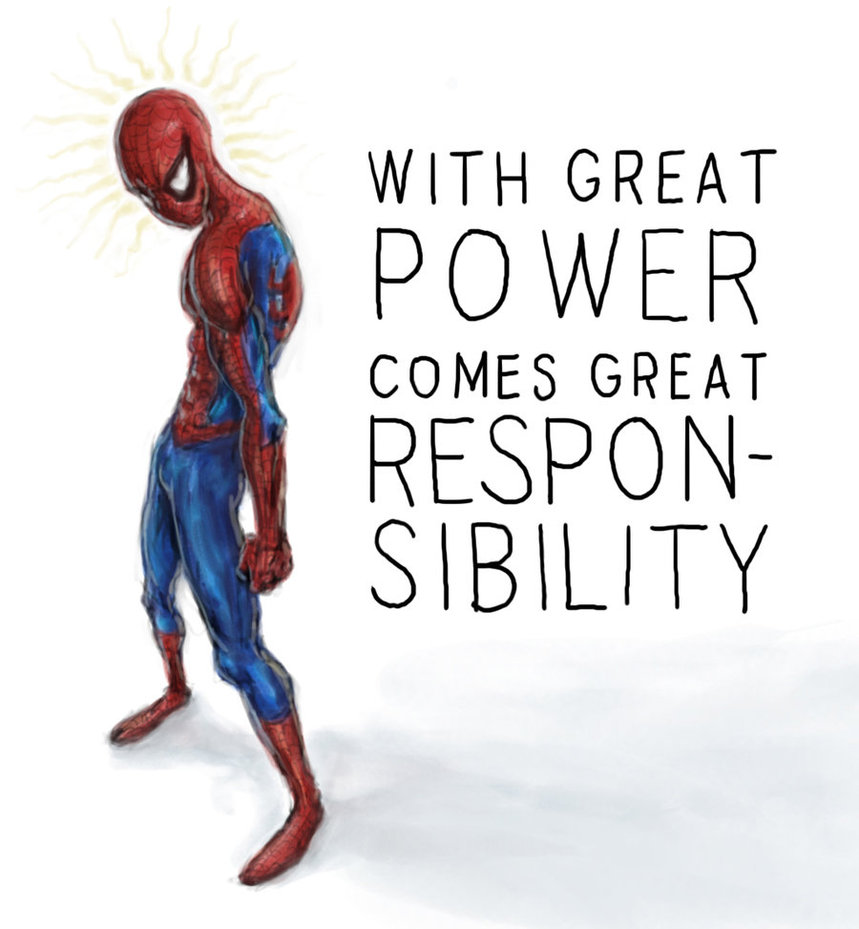
\includegraphics[width=\linewidth]{spiderman.jpg}
  \label{fig:spiderman}
\end{marginfigure}

Rewriting history is a great way of cleaning one's work before pushing, but should not be used a posteriori on an important branch (master, develop). \marginnote{Implied here: it's still OK to force push your personal feature branches, but don't let it become a habit} Git takes care of guarding you from such actions by requiring the \texttt{--force} option to the \texttt{push} command whenever it detects a change in an existing branche's history.

If you ever have doubts about when it is ok or not to rewrite history, use \textbf{this simple rule: do not modify history pushed on a shared repository.}

\section{Rewriting History}
Git gives lots of power to the user and allows to rewrite the history.
This can be \textbf{rewording} commit messages, \textbf{combining} commits, \textbf{splitting} a large commit into smaller ones, \textbf{deleting} a commit, \textbf{reordering} commits, changing the \textbf{date and authoring} information, etc.

\subsection{Amending the last commit}
The simplest form of history modification is changing the last commit:

\begin{lstlisting}[style=BashInputStyle]
  $ git commit --amend
\end{lstlisting}

This command opens up the last commit message, and allows you to alter the message.
It also takes whatever was added to the staging area (via \texttt{git add}) and combines it with the previous commit, instead of creating a new commit.
Thus, this is for both \textbf{rewording the last commit} and \textbf{altering the contents of the last commit}.

Let's reword the last commit message of the master branch of the lesson1 repository:

\begin{lstlisting}[style=BashInputStyle]
  $ git clone git@gitlab.server.com:login/lesson1
  $ cd lesson1
  $ git checkout master # not necessary
  $ git log --oneline
  $ gitk --all
  $ git commit --amend -m "New message"
  $ git log --oneline
  $ gitk --all
\end{lstlisting}

\begin{figure*}%
  \centering
  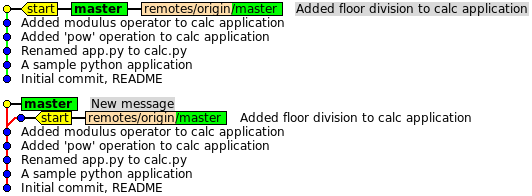
\includegraphics[width=0.85\linewidth]{gitcommit-amend.png}
  \label{fig:gitcommit-amend}
  \caption{Before (top) and after (bottom) amending the last commit message}
\end{figure*}

The output of gitk at the 2 steps is shown in Figure \ref{fig:gitcommit-amend}.
We can see that ammending the commit creates a divergence between out local master branch's history and that of the remote's.
The change in history means \textbf{you cannot git push} without the \texttt{--force} option. \marginnote{Since a commit's HASH reflects the state of the working tree and all commit-related metainfo (author, commit message, date...) changing any of these is considered a modification}
In fact, doing so will raise an error because git refuses to push work on a branch which does not pick up from the branch's last commit in its exact state, (HASH-wise).

\subsection{More thorough history modifications with interactive rebase}
Amending the last commit only scratches the surface of history modifications.
A more general and powerful command to edit history is the interactive rebase command.

To \textbf{rebase} the HEAD on a certain tree-ish, means to:

\begin{enumerate} 
 \item{rewind both the HEAD and the specified tree-ish until obtaining a common point in history}
 \item{apply the commits belonging to HEAD, missing from the tree-ish on top of that tree-ish}
 \item{continuously move the current HEAD to the latest commit as the patches are applied}
\end{enumerate}

This is a very general command used in different contexts.
When applying each commit on the new base, we can tell git to perform extra operations are each step when invoking \textbf{rebase in interactive mode}.
This is particularly convenient for rewriting history: we simply rebase the current HEAD on a commit in the direct history.

Suppose we wanted to alter the commit messages of HEAD\textasciitilde1 and HEAD\textasciitilde2, we would do:
\marginnote{Reminder: HEAD\textasciitilde n is a shortcut to designate the n+1 th last commit (i.e. n commits behind the latest commit)}
\begin{lstlisting}[style=BashInputStyle]
  $ git rebase -i HEAD~3
\end{lstlisting}

The means we take the HEAD, and rebase it on a commit which is 3 commits away.
This will undo HEAD, HEAD\textasciitilde1 and HEAD\textasciitilde2, and apply them on top of HEAD\textasciitilde3 in reverse order (HEAD\textasciitilde2, HEAD\textasciitilde1, HEAD). \marginnote{without the -i option, this command has no effect.}
With the -i option, an editor pops up to prompt us if we want to take any action when picking each commit:

\begin{lstlisting}[style=BashInputStyle]
  pick 21471dd Added 'pow' operation to calc application
  pick 511d31d Added modulus operator to calc application
  pick 87854e9 New message
\end{lstlisting}

We will ask to edit 2 of the commits by replacing the 'pick' header of the appropriate lines:

\begin{lstlisting}[style=BashInputStyle]
  edit 21471dd Added 'pow' operation to calc application
  edit 511d31d Added modulus operator to calc application
  pick 87854e9 New message
\end{lstlisting}

When closing the editor, git will take each commit from top to bottom and perform the requested action.
The first action is to pick and edit 21471dd, so git will stop immediately to allow the user to amend the commit:

\begin{lstlisting}[style=BashInputStyle]
Stopped at 21471dd... Added 'pow' operation to calc application
You can amend the commit now, with

	git commit --amend

Once you are satisfied with your changes, run

	git rebase --continue
\end{lstlisting}

Let's follow Git's suggestions and amend the commit and continue the rebase operation:

\begin{lstlisting}[style=BashInputStyle]
git commit --amend -m "New commit message 1"
git rebase --continue
\end{lstlisting}

We get a similar message as before saying Git has stopped on commit 511d31d.
Again, we amend and continue the rebase:

\begin{lstlisting}[style=BashInputStyle]
git commit --amend -m "New commit message 2"
git rebase --continue
\end{lstlisting}

Git will automatically end the rebase operation when there are not more inputs required.
Our last commit is in 'pick' mode, so it is automatically picked without a user prompt.
The final history after the first amend operation and this rebase and its relationship to the remote master branch is shown in Figure \ref{fig:gitrebase-amend}.

\begin{figure*}%
  \centering
  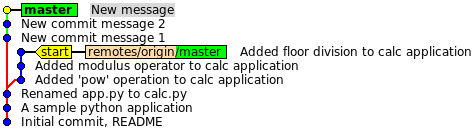
\includegraphics[width=0.75\linewidth]{gitrebase-amend.png}
  \label{fig:gitrebase-amend}
  \caption{Result of amending the last 3 commit messages}
\end{figure*}

\noindent We have covered the general mechanism of git rebase in interactive mode. 
We will now have a small preview of more advances operation which can be done with rebase.
First, let's undo our changes by reset our local master branch to the state of origin/master:

\begin{lstlisting}[style=BashInputStyle]
  git reset --hard origin/master
\end{lstlisting}

\noindent \textbf{Squashing Commits}.
A number of small commits can be combined into one.

This is done using the \textbf{squash} keyword in the git rebase editor.
Let's combine HEAD~1 and HEAD~2:

\begin{lstlisting}[style=BashInputStyle]
  $ git rebase -i HEAD~3
\end{lstlisting}

This time, we modify the rebase editor like the following:
\marginnote{The \textbf{squash} action combines a commit with the previous one, so we need to add squash to the \textbf{lower} element of a pair of commits}
\begin{lstlisting}[style=BashInputStyle]
  pick 21471dd Added 'pow' operation to calc application
  squash 511d31d Added modulus operator to calc application
  pick 87854e9 New message
\end{lstlisting}

When rebasing this, Git first picks 21471dd, then amends it with 511d31d.
An editor opens promoting for the new commit message of the combined commit:
\marginnote{In fact, the squashing in Git is pretty smart: if you squash more than 2 consecutive commits, they will all appear together in this step.}
\begin{lstlisting}[style=BashInputStyle]
# This is a combination of 2 commits.
# The first commit's message is:

Added 'pow' operation to calc application

# This is the 2nd commit message:

Added modulus operator to calc application
\end{lstlisting}

Let's modify it to:

\begin{lstlisting}[style=BashInputStyle]
Added 'pow' and 'modulus' operators
\end{lstlisting}

\begin{lstlisting}[style=BashInputStyle]
  $ git rebase --continue
\end{lstlisting}

The rebase will complete and our new history is shown in Figure \ref{fig:gitrebase-squash}

\begin{figure*}%
  \centering
  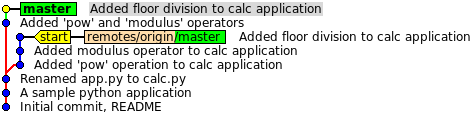
\includegraphics[width=0.75\linewidth]{gitrebase-squash.png}
  \label{fig:gitrebase-squash}
  \caption{Result of a squash in a git rebase}
\end{figure*}

Let's reset our branch again before the next part:

\begin{lstlisting}[style=BashInputStyle]
  git reset --hard origin/master
\end{lstlisting}

\noindent \textbf{Splitting a commit into smaller commits}
Splitting a large commit into smaller ones is also possible, but slightly trickier.
The keyword to use in the interactive rebase editor is \textbf{edit}, just like for editing the commit message.
Suppose we want to split the commit implementing the modulus operation.
We can rebase upto HEAD\textasciitilde2:

\begin{lstlisting}[style=BashInputStyle]
  $ git rebase -i HEAD~2
\end{lstlisting}

In the rebase editor, we \textbf{edit} 511d31d:
\begin{lstlisting}[style=BashInputStyle]
  edit 511d31d Added modulus operator to calc application
  pick 87854e9 New message
\end{lstlisting}

Git will stop after picking 511d31d.
\textbf{The tricky part:} Git has already picked the commit as a whole, the pause is there to add stuff to the staging area and/or edit the commit message.
So how to split it up into smaller ones?
\marginnote{yes, a reset within a rebase operation is allowed}
The user must now \textbf{reset} on HEAD\textasciitilde1, which undoes the last commit, the one Git has just picked, and sets to modified state all the modifications of the commit.

\begin{lstlisting}[style=BashInputStyle]
  $ git reset HEAD~1
\end{lstlisting}

\marginnote{remember how useful git add -p is for staging partial information}
You can now \textbf{git add} the modifications partially, commit, stage more, commit again, etc, until everything has been staged and committed:

\begin{lstlisting}[style=BashInputStyle]
  $ git add -p
  # stage part of the modifications
  $ git commit -m "modulus implementation, phase 1"
  $ git add -p
  # stage part of the modifications
  $ git commit -m "modulus implementation, phase 2"
  $ git rebase --continue
\end{lstlisting}

The local master branch will now contain the split commit:

\begin{figure*}%
  \centering
  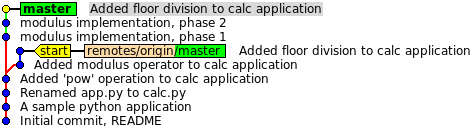
\includegraphics[width=0.75\linewidth]{gitrebase-split.png}
  \label{fig:gitrebase-split}
  \caption{Result of a split in a git rebase}
\end{figure*}

\noindent \textbf{Deleting and Reordering commits}

Finally, it's possible to delete and reorder commits.
To do so, simply delete and reorder lines in the interactive rebase editor.
This is left as exercice.

\bibliography{../common/refs}
\bibliographystyle{plainnat}

\end{document}